\section{\hspace{1em} Числени симулации}
\begin{frame}[t]{Таблица със стойности на параметри}
  % \begin{table}
  % \hskip-0.65cm
  \begin{footnotesize}
      \begin{tabular}{ |c ||c c c c c c|  }
        % \hhline{~------}
        \hline
        \multirow{2}{*}{Параметър}& \multicolumn{2}{c}{Набор 1}& \multicolumn{2}{c}{Набор 2} & \multicolumn{2}{c|}{Набор 3}\\
        & М. 1 & М. 2 & М. 1 & М. 2 & М. 1 & М. 2\\
        \hline
        % \hhline{~------}
        $\beta_{vh}$ & \multicolumn{2}{c}{$0.5$} & \multicolumn{2}{c}{$0.5$}  & \multicolumn{2}{c|}{$0.5$}\\
        $\beta_{hv}$ & \multicolumn{2}{c}{$0.1$} & \multicolumn{2}{c}{$0.1$} & \multicolumn{2}{c|}{$0.1$}\\
        $a_i$ & $0.12$ & $0.18$ & $0.158$ & $0.159$ & $0.15$ & $0.24$\\
        $M_i$ & $6 \times 10^7$ & $1.6 \times 10^8$ & $1.7 \times 10^7$ & $3 \times 10^7$ & $7.3 \times 10^6$ & $4.7 \times 10^6$\\
        $\mu_i$ & $0.048$ & $0.067$ & $0.032$ & $0.046$ & $0.04$ & $0.034$\\
        $\tau$ & \multicolumn{2}{c}{$10$} & \multicolumn{2}{c}{$10$} & \multicolumn{2}{c|}{$10$}\\
        $N_i$ & $8 \times 10^6$ & $2 \times 10^7$ & $9.4 \times 10^6$ & $4.5 \times 10^6$ & $7.6 \times 10^5$ & $4 \times 10^6$\\
        $\gamma_i$ & $0.071$ & $0.071$ & $0.063$ & $0.058$ & $0.074$ & $0.062$\\
        $p_{ij}$ & \multicolumn{6}{c|}{различни ($p_{i1}+p_{i2}=1$)}\\
        $\kappa$ & \multicolumn{2}{c}{$0.44$} & \multicolumn{2}{c}{$0.37$} & \multicolumn{2}{c|}{$0.38$}\\
        $\bar{u}_i$ & $0.15$ & $0.3$ & $0.39$ & $0.12$ & $0.35$ & $0.3$\\
        $\bar{I}_i$ & $0.1$ & $0.14$ & $0.065$ & $0.12$ & $0.09$ & $0.09$\\
        \hline
      \end{tabular}
    \end{footnotesize}
    %   \caption{Таблица със стойностите на параметрите}
    %   \label{tbl:ParameterValues}
    % \end{table}
\end{frame}

\begin{frame}[t]{Ендемичното състояние спрямо мобилността}
  \begin{figure}[h]
    \centering
    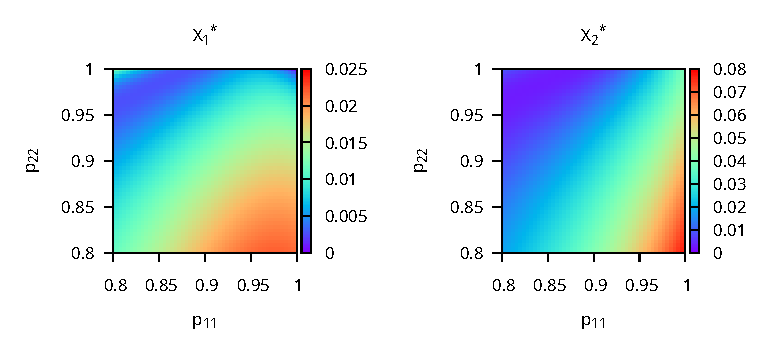
\includegraphics[width=\textwidth]{equilibrium-poster.pdf}
    \caption{Пропорция заразени жители при равновесие на \eqref{eq:TheDimensionlessProblem}} при $\boldsymbol{u}(t) \equiv \bar{\boldsymbol{u}}$ с параметрите от набор 1.
    \label{fig:EquilibriumPoints-poster}
  \end{figure}
\end{frame}

\begin{frame}[t]{Ендемичното състояние спрямо мобилността}
  \begin{figure}[h]
    \centering
    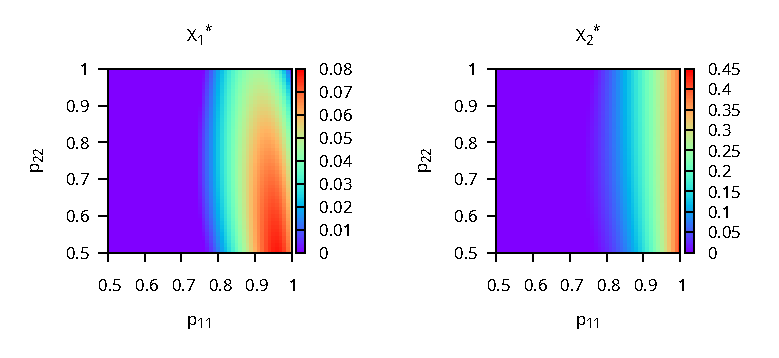
\includegraphics[width=\textwidth]{equilibrium-03-19-16-12-04.pdf}
    \caption{Пропорция заразени жители при равновесие на \eqref{eq:TheDimensionlessProblem}} при $\boldsymbol{u}(t) \equiv \bar{\boldsymbol{u}}$ с параметрите от набор 2.
    \label{fig:EquilibriumPoints-03-19-16-12-04}
  \end{figure}
\end{frame}

\begin{frame}[t]{Ендемичното състояние спрямо мобилността}
  \begin{figure}[h]
    \centering
    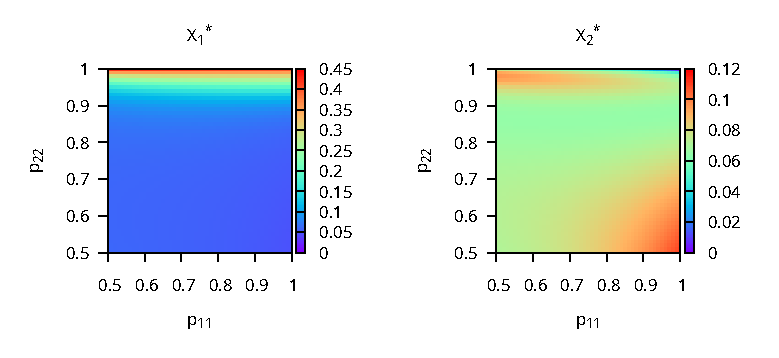
\includegraphics[width=\textwidth]{equilibrium-03-19-16-58-19.pdf}
    \caption{Пропорция заразени жители при равновесие на \eqref{eq:TheDimensionlessProblem}} при $\boldsymbol{u}(t) \equiv \bar{\boldsymbol{u}}$ с параметрите от набор 3.
    \label{fig:EquilibriumPoints-03-19-16-58-19}
  \end{figure}
\end{frame}

\begin{frame}[t]{Числено приближение на $V(\bar{\boldsymbol{I}}, \bar{\boldsymbol{u}})$ }
  \begin{table}[H]
    \centering
    \begin{tabular}{ | c| c c c c|}
      \hline
      \backslashbox{$p_{22}$}{$p_{11}$}& 0.8 & 0.85 & 0.9 & 0.95 \\
      \hline
      0.95 & 3.427 & 3.447 & 3.467 & 3.486\\
      0.9 & 3.468 & 3.487 & 3.507 & 3.527\\
      0.85 & 3.498 & 3.517 & 3.536 & 3.554\\
      0.8 & 3.519 & 3.540 & 3.559 & 3.580\\
      \hline
    \end{tabular}
    \caption{4-мерната мярка на $V(\bar{\boldsymbol{I}}, \bar{\boldsymbol{u}})$ за параметрите от набор 1. Стойността при случая без мобилност е взета за референтна.}
    \label{tbl:ViabilityKernel-poster}
  \end{table}
\end{frame}

\begin{frame}[t]{Динамика за $\boldsymbol{z}_0 \in V(\bar{\boldsymbol{I}}, \bar{\boldsymbol{u}})$}
  \begin{figure}[h]
    \centering
    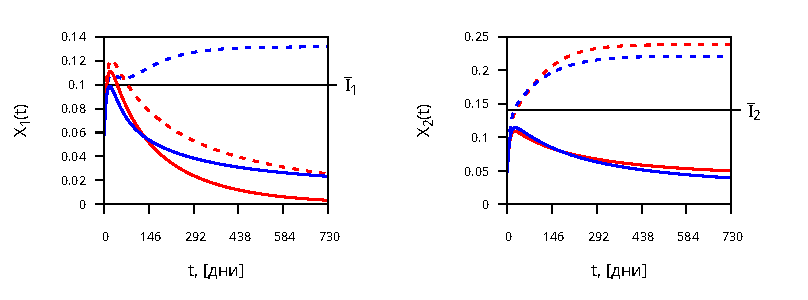
\includegraphics[width=\textwidth]{solution-poster.pdf}
    \caption{
      Решението на \eqref{eq:TheDimensionlessProblem} с параметрите от набор 1 и $\boldsymbol{z}_0=(0.0572, 0.048, 0.052, 0.044)^T$.\\
      \dashuline{Пунктирано}: $\boldsymbol{u}(t) \equiv \pmb{0}$, \underline{плътно}: $\boldsymbol{u}(t) \equiv \bar{\boldsymbol{u}}$.\\
      \textcolor{red}{Червено}: $p_{11}=p_{22}=1$, \textcolor{blue}{синьо}: $p_{11}=p_{22}=0.85$.
    }
    \label{fig:Solution-poster}
  \end{figure}
\end{frame}

\begin{frame}[t]{Динамика за $\boldsymbol{z}_0 \notin V(\bar{\boldsymbol{I}}, \bar{\boldsymbol{u}})$}
  \begin{figure}[h]
    \centering
    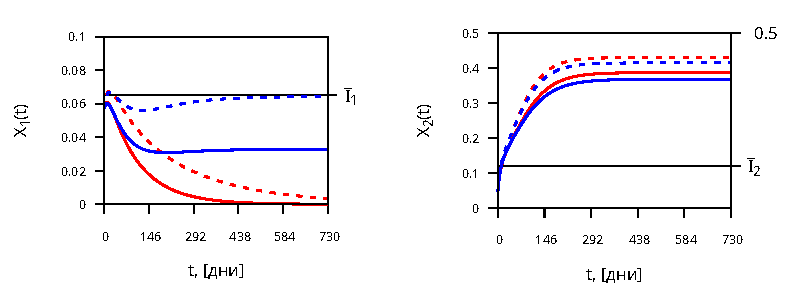
\includegraphics[width=\textwidth]{solution-03-19-16-12-04.pdf}
    \caption{
      Решението на \eqref{eq:TheDimensionlessProblem} с параметрите от набор 2 и $\boldsymbol{z}_0=(0.0572, 0.048, 0.052, 0.044)^T$.\\
      \dashuline{Пунктирано}: $\boldsymbol{u}(t) \equiv \pmb{0}$, \underline{плътно}: $\boldsymbol{u}(t) \equiv \bar{\boldsymbol{u}}$.\\
      \textcolor{red}{Червено}: $p_{11}=p_{22}=1$, \textcolor{blue}{синьо}: $p_{11}=0.99, p_{22}=0.9$.
    }
    \label{fig:Solution-03-19-16-12-04}
  \end{figure}
\end{frame}

\begin{frame}[t]{Динамика спрямо мобилността}
  \begin{figure}[h]
    \centering
    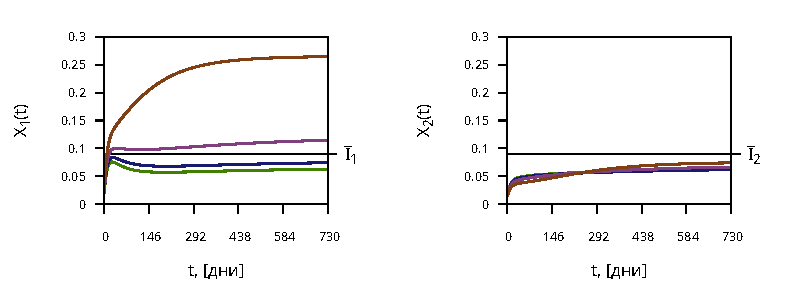
\includegraphics[width=\textwidth]{solution-03-19-16-58-19-bold.pdf}
    \caption{
      Решението на \eqref{eq:TheDimensionlessProblem} с параметрите от набор 3, $\boldsymbol{z}_0=(0.02, 0.015, 0.04, 0.03)^T$, $\boldsymbol{u}(t) \equiv \bar{\boldsymbol{u}}$, фиксирано $p_{11}=0.93$, а различно $p_{22}$.\\
      \textcolor{Sienna4}{кафяво}: $p_{22}=0.97$,\\
      \textcolor{Orchid4}{лилаво}: $p_{22}=0.92$,\\
      \textcolor{MidnightBlue}{синьо}: $p_{22}=0.88$,\\
      \textcolor{DarkChartreuse}{зелено}: $p_{22}=0.85$.\\
    }
    \label{fig:Solution-03-19-16-58-19}
  \end{figure}
\end{frame}
